\begin{savequote}[8cm]
A process cannot be understood by stopping it. Understanding must move with the flow of the process, must join it and flow with it. (First Law of Mentat)
  \qauthor{--- Frank Herbert, Dune}
\end{savequote}
%Edsger W. Dijkstra, How do we tell truths that might hurt? (1975).

\chapter{Tools for design and simulation of individual modules}\label{sec:toolsForIndMod}

\minitoc


Simulating the structure and dynamics of individual DNA origami modules has been possible for a while, but my aim with this project has been to make such simulations more accessible and easy to use and analyse.

%This is accomplished as I develop new tools and scripts while learning about the simulation methods and the designs that various laboratories are interested in.

This chapter describes the currently available tools for simulation and design of individual module structures. DNA and RNA structures can be digitally represented in many different formats, for many different uses, and with different levels of coarse-graining. 

The following sections cover my results over the last year, investigating methods for converting designs into the oxDNA/RNA format and for visualising and analysing the simulation results.

\section{Simulation tools}
Simulating a structure can provide insight to understand experimental results, but can also guide decisions at the design stage. Different models

\subsection{All-atom simulation}
Simulation tools such as NAMD\cite{NAMDphillips2005scalable}, use force fields such as AMBER\cite{AMBERcornell1996second} and CHARMM \cite{brooks1983charmm} that model interactions between individual atoms. While it is possible to perform atomistic simulations of large DNA origami structures\cite{yoo2013situ}, the simulations take a long time to run and it is unknown how well the models represent DNA thermodynamics \cite{sengar2021primer}.

\subsection{oxDNA/RNA}
In 2010, a the coarse-grained simulation software called oxDNA was introduced by Thomas Ouldridge \cite{ouldridge2010dna}. It simulates DNA on the level of nucleotides and has been shown to model complex origami devices with a generally good agreement with experimental data \cite{sharma2017characterizing}. In 2014, the DNA model was extended to include RNA by Petr {\v{S}}ulc \cite{vsulc2014nucleotide}, showing its ability to model a set of common RNA motifs. 

Molecular Dynamics (MD) and Monte Carlo (MC) simulation techiniques.

OxDNA was joined by cogli1 for trajectory visualisation.


% Mention ANM model by Jonah!!!

While oxDNA can be very useful for modelling a structure, it has traditionally not been very accessible for experimentalists. % mention web server

\begin{figure}[h]
\begin{center}
    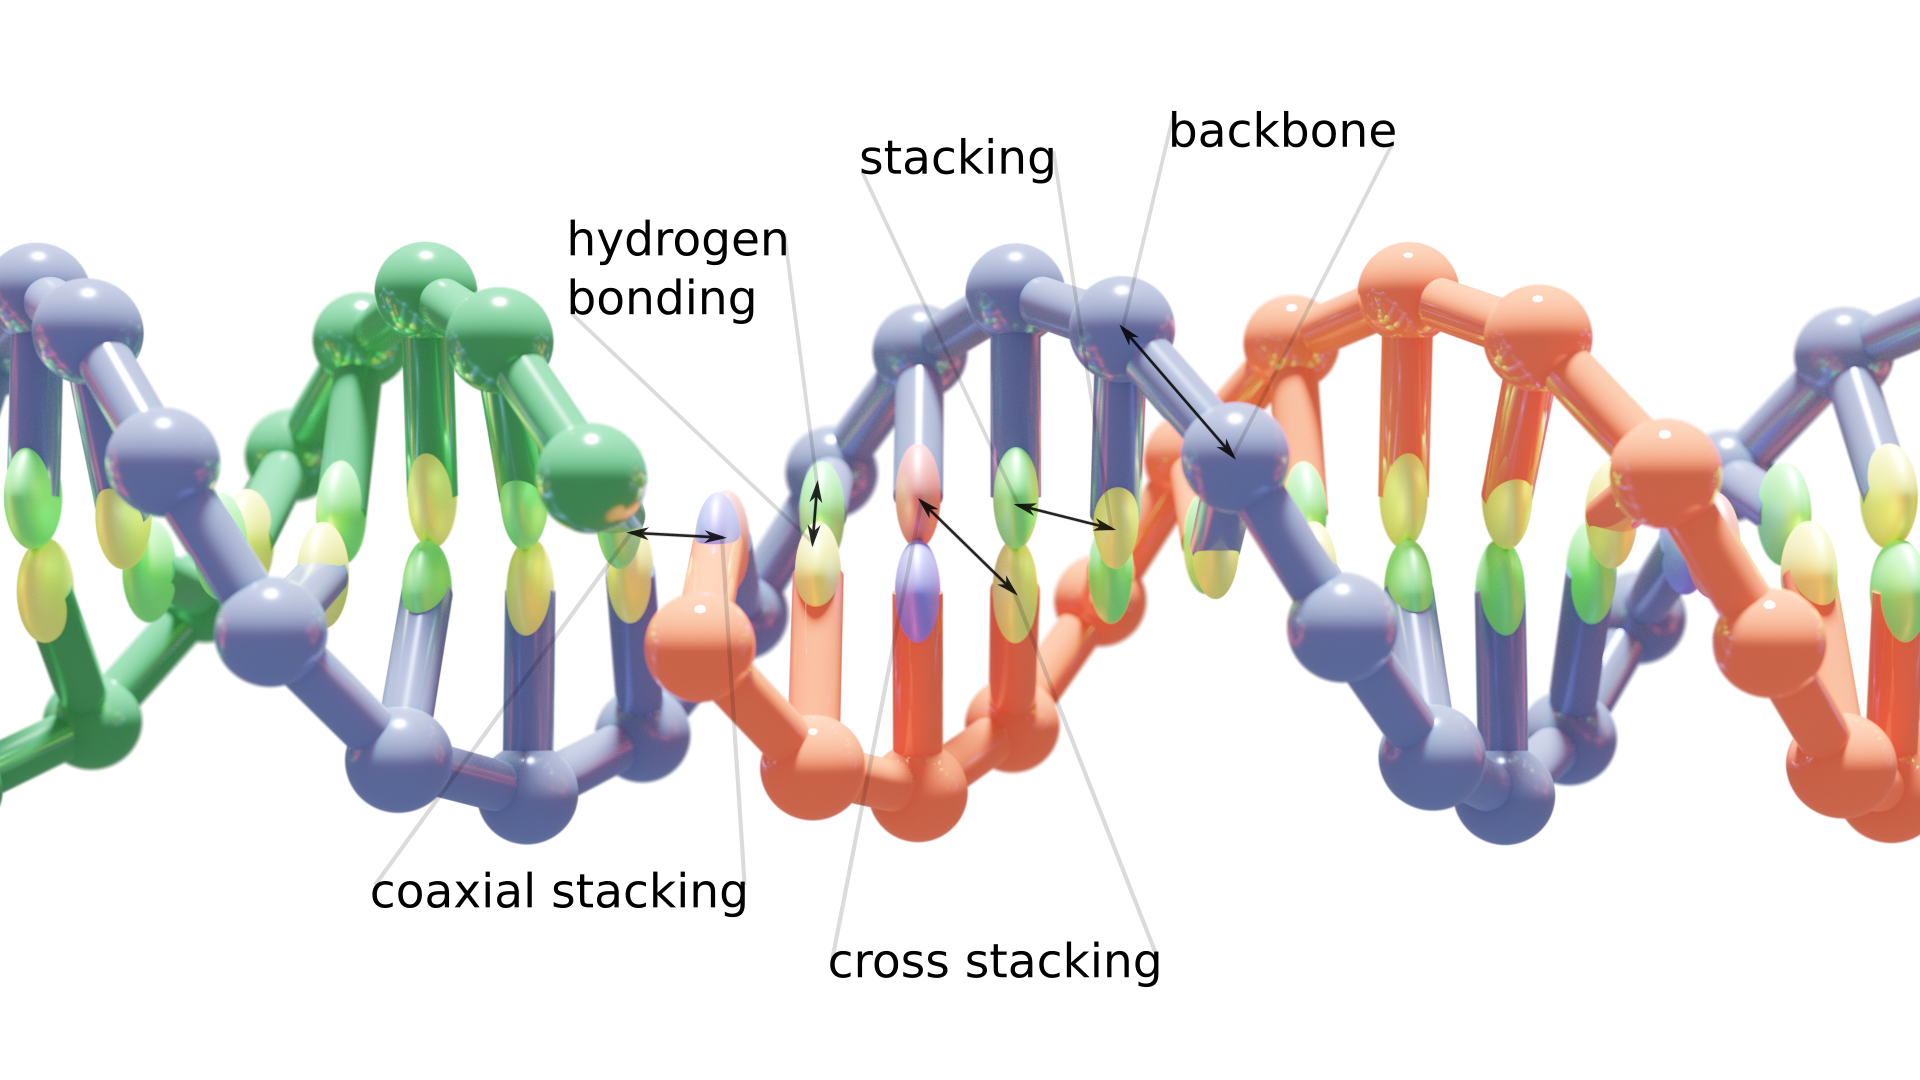
\includegraphics[width=\textwidth]{figures/oxdna_annot.png}
    \caption{The oxDNA model}
    \label{fig_oxDNA}
    \end{center}
\end{figure}

\subsection{mrDNA}
Another promising feature of mrdna is that it has a spline-based helix representation and is implemented in python. This enables users to easily script edits to the stucture, translating and rotating parts of it before starting the simulation. Thus, topological issues or over-stretched bonds can, with some skill, be resolved even before starting to simulate. I did, based on this, also create a rudimentary interactive editor interface to mrdna, but it would need a lot of refinement to be externally usable.

\subsection{Cando}

Cando is a finite element modelling framework\cite{kim2012cando} available through a web server at \url{https://cando-dna-origami.org}. DNA double helices are modelled as elastic rods (connected by rigid crossovers) that stretch, twist and bend in line with experimental measurements.

\section{Design tools}\label{sec:design_tools}
Designing a DNA origami structure by hand would be a very labourious task for anything but the most simple design. As such, a host of computer-aided design tools have been introduced over the years to make things easier. This section will cover some of the more popular examples.

\subsection{Lattice-based design tools}
The caDNAno design tool \cite{cadnano} and the web-based scadnano\cite{scadnano} it inspired, allows the user to design DNA origami on a lattice of parallel helices.
\subsubsection{caDNAno}
CaDNAno \cite{cadnano} was introduced in 2009 as a way to simplify 3D DNA origami designs. It has a graphical user interface where the designer can place virtual helices on a lattice (either hexagonal or square). The helices can then be filled in with strands and connected using crossovers at logical positions.
\subsubsection{Scadnano}

\subsection{Top-down shape converters}

\subsubsection{BSCOR}\label{sec:bscor}
\subsubsection{DAEDAULS/PERDIX}
ATHENA? %https://www.biorxiv.org/content/10.1101/2020.02.09.940320v1.full.pdf
\subsubsection{Triangulated truss structures}
% M. Matthies
% https://pubs.acs.org/doi/abs/10.1021/acs.nanolett.6b00381

\subsection{Free-form or hybrid tools}

\subsubsection{Tiamat}
Tiamat is an early free-form design tool

\subsubsection{vHelix}

\subsubsection{Adenita}
A final option for structure editing is Adenita \cite{miao_tvcg_2018}. So far, a version has only been released for beta testers and unfortunately, they do not yet support Linux. Still, after talking to Haichao Miao at the Nantech2019 conference, Adenita sounds like it could become a valuable off-lattice tool for designing and editing DNA nanostructures, with import options from caDNAno and export to oxDNA.

\subsubsection{MagicDNA}
Another method of solving topological issues through rigid-body manipulation was used by Chao-Min Huang \cite{huang2019uncertainty}. The tool used is not public, so I have not been able to examine it, but the supplementary material of the article shows them using a Matlab script to interactively move and rotate the helix bundles (treated as rigid bodies) into a desired configuration with less stretched bonds.

\subsubsection{oxView}
The oxView application was developed as part of this thesis project and will be described more in the following chapter.